% ============================================================
%  NERC RELIABILITY COORDINATOR (RC) CERTIFICATION EXAM
%  COMPREHENSIVE STUDY GUIDE
%  Ricardo Barbosa — 2026
% ============================================================
\documentclass[12pt,twoside,openright]{memoir}

% ── Encoding & fonts ─────────────────────────────────────────
\usepackage[T1]{fontenc}
\usepackage[utf8]{inputenc}
\usepackage{lmodern}
\usepackage{microtype}
\usepackage{palatino}
\usepackage[scaled=0.85]{beramono}

% ── Page geometry ────────────────────────────────────────────
\usepackage[
  top=1.25in, bottom=1.25in,
  inner=1.5in, outer=1.0in,
  marginparwidth=0.8in, marginparsep=0.1in
]{geometry}

% ── Colors ───────────────────────────────────────────────────
\usepackage[dvipsnames,svgnames,x11names]{xcolor}
\definecolor{nercnavy}{HTML}{0D2137}
\definecolor{nercblue}{HTML}{1565C0}
\definecolor{nerccyan}{HTML}{0097A7}
\definecolor{nercorange}{HTML}{E65100}
\definecolor{nercgreen}{HTML}{2E7D32}
\definecolor{nercred}{HTML}{C62828}
\definecolor{nercyellow}{HTML}{F9A825}
\definecolor{rowlight}{HTML}{EFF6FF}
\definecolor{rowdark}{HTML}{DBEAFE}
\definecolor{codebg}{HTML}{F8F9FA}
\definecolor{frameborder}{HTML}{455A64}
\definecolor{covergray}{HTML}{ECEFF1}
\definecolor{warnbg}{HTML}{FFF3E0}
\definecolor{alertbg}{HTML}{FFEBEE}

% ── Graphics & TikZ ──────────────────────────────────────────
\usepackage{graphicx}
\usepackage{tikz}
\usetikzlibrary{positioning,shapes.geometric,arrows.meta,decorations.pathreplacing,
                matrix,fit,backgrounds,calc,patterns,shadows.blur}
\usepackage{pgfplots}
\pgfplotsset{compat=1.18}

% ── Tables ───────────────────────────────────────────────────
\usepackage{booktabs}
\usepackage{tabularx}
\usepackage{array}
\usepackage{multirow}
\usepackage{colortbl}
\newcolumntype{L}[1]{>{\raggedright\arraybackslash}p{#1}}
\newcolumntype{C}[1]{>{\centering\arraybackslash}p{#1}}
\newcolumntype{R}[1]{>{\raggedleft\arraybackslash}p{#1}}

% ── Callout boxes (tcolorbox) ─────────────────────────────────
\usepackage[most,listings]{tcolorbox}

\newtcolorbox{keyconcept}[1][]{
  enhanced, breakable,
  colback=nercblue!8, colframe=nercblue, arc=4pt,
  fonttitle=\bfseries\sffamily\color{white}, title={Key Concept},
  attach boxed title to top left={yshift=-2mm, xshift=6mm},
  boxed title style={colback=nercblue, arc=3pt},
  #1
}

\newtcolorbox{warningbox}[1][]{
  enhanced, breakable,
  colback=warnbg, colframe=nercorange, arc=4pt,
  fonttitle=\bfseries\sffamily\color{white}, title={WARNING},
  attach boxed title to top left={yshift=-2mm, xshift=6mm},
  boxed title style={colback=nercorange, arc=3pt},
  #1
}

\newtcolorbox{examtip}[1][]{
  enhanced, breakable,
  colback=nercgreen!6, colframe=nercgreen, arc=4pt,
  fonttitle=\bfseries\sffamily\color{white}, title={Exam Tip},
  attach boxed title to top left={yshift=-2mm, xshift=6mm},
  boxed title style={colback=nercgreen, arc=3pt},
  #1
}

\newtcolorbox{formulabox}[2][]{
  enhanced, breakable,
  colback=nercnavy!5, colframe=nercnavy, arc=4pt,
  fonttitle=\bfseries\sffamily\color{white}, title={Formula: #2},
  attach boxed title to top left={yshift=-2mm, xshift=6mm},
  boxed title style={colback=nercnavy, arc=3pt},
  #1
}

\newtcolorbox{criticalbox}[1][]{
  enhanced, breakable,
  colback=alertbg, colframe=nercred, arc=4pt,
  fonttitle=\bfseries\sffamily\color{white}, title={Critical — Immediate Action Required},
  attach boxed title to top left={yshift=-2mm, xshift=6mm},
  boxed title style={colback=nercred, arc=3pt},
  #1
}

% ── Code listings ─────────────────────────────────────────────
\usepackage{listings}
\lstdefinestyle{nercstyle}{
  basicstyle=\ttfamily\small,
  backgroundcolor=\color{codebg},
  frame=single, framerule=0.5pt, rulecolor=\color{frameborder},
  breaklines=true, keepspaces=true,
  xleftmargin=10pt, xrightmargin=10pt,
  aboveskip=6pt, belowskip=6pt,
  showstringspaces=false
}
\lstset{style=nercstyle}

% ── Headers & footers ────────────────────────────────────────
\usepackage{fancyhdr}
\pagestyle{fancy}
\fancyhf{}
\fancyhead[LE]{\small\sffamily\color{nercblue}\leftmark}
\fancyhead[RO]{\small\sffamily\color{nercblue}\rightmark}
\fancyfoot[LE,RO]{\small\sffamily\thepage}
\fancyfoot[CO,CE]{\small\sffamily\color{gray}NERC RC Certification Exam Study Guide}
\renewcommand{\headrulewidth}{0.4pt}
\renewcommand{\footrulewidth}{0.2pt}

% ── Hyperref ──────────────────────────────────────────────────
\usepackage[
  colorlinks=true,
  linkcolor=nercblue,
  urlcolor=nerccyan,
  citecolor=nercgreen,
  pdfauthor={Ricardo Barbosa},
  pdftitle={NERC Reliability Coordinator (RC) Certification Exam Study Guide},
  pdfsubject={NERC RC Operator Certification},
  pdfkeywords={NERC, RC, Reliability Coordinator, power systems, certification, BAL, EOP, IRO, TOP, VAR},
  bookmarks=true, bookmarksnumbered=true
]{hyperref}

% ── Misc ──────────────────────────────────────────────────────
\usepackage{enumitem}
\usepackage{amsmath}
\usepackage{amssymb}
\usepackage{soul}
\usepackage{mdframed}

% ── Memoir chapter style ──────────────────────────────────────
\makechapterstyle{nerc}{%
  \renewcommand{\chapnamefont}{\normalfont\Large\sffamily\color{nercblue}}
  \renewcommand{\chapnumfont}{\normalfont\fontsize{56}{56}\bfseries\sffamily\color{nercblue!25}}
  \renewcommand{\chaptitlefont}{\normalfont\Huge\bfseries\sffamily\color{nercnavy}}
  \renewcommand{\printchapternum}{%
    \begin{tikzpicture}[remember picture]
      \node[fill=nercblue!10, rounded corners=6pt,
            inner sep=8pt, minimum width=3cm]{%
        \chapnumfont\thechapter};
    \end{tikzpicture}
  }
  \renewcommand{\afterchapternum}{\par\vspace{4pt}}
  \renewcommand{\afterchaptertitle}{%
    \par\vspace{4pt}
    
\begin{tikzpicture}
      \draw[nercblue, line width=2.5pt] (0,0) -- (\textwidth,0);
      \draw[nercorange, line width=1.2pt] (0,-3pt) -- (3cm,-3pt);
    \end{tikzpicture}
    \par\vspace{16pt}
  }
}
\chapterstyle{nerc}

\setsecheadstyle{\large\bfseries\sffamily\color{nercblue}}
\setsubsecheadstyle{\normalsize\bfseries\sffamily\color{nercnavy}}
\setsubsubsecheadstyle{\normalsize\itshape\sffamily\color{nercnavy}}

% ── Helper macros ─────────────────────────────────────────────
\newcommand{\std}[1]{\texttt{\textbf{#1}}}
\newcommand{\Hz}[1]{#1\,Hz}
\newcommand{\MW}[1]{#1\,MW}
\newcommand{\MVAR}[1]{#1\,MVAR}

% ============================================================
\begin{document}

% ── Cover Page ────────────────────────────────────────────────
\begin{titlingpage}
  \pagecolor{nercnavy}
  \color{white}
  \vspace*{2cm}

  \begin{tikzpicture}[remember picture, overlay]
    \fill[nercblue!30, opacity=0.3]
      (-2, -5) rectangle (18, 12);
    \draw[nerccyan, line width=3pt, opacity=0.5]
      (-2, 6) -- (18, 6);
  \end{tikzpicture}

  \begin{center}
    {\fontsize{11}{13}\selectfont\sffamily\color{nerccyan}
      NORTH AMERICAN ELECTRIC RELIABILITY CORPORATION}

    \vspace{0.4cm}
    {\fontsize{36}{40}\selectfont\bfseries\sffamily
      NERC RC CERTIFICATION\\
      EXAM STUDY GUIDE}

    \vspace{0.5cm}
    
\begin{tikzpicture}
      \draw[nercorange, line width=2pt] (0,0) -- (12cm,0);
    \end{tikzpicture}

    \vspace{0.5cm}
    {\fontsize{18}{22}\selectfont\sffamily\color{nercyellow}
      Reliability Coordinator (RC)\\
      Comprehensive Exam Preparation}

    \vspace{1.5cm}
    {\fontsize{13}{16}\selectfont\sffamily\color{white!80}
      Covering All 10 Study Chapters:\\
      BAL · EOP · INT · IRO · TOP · VAR · PRC · FAC · COM · MOD}

    \vspace{2cm}
    {\fontsize{14}{17}\selectfont\sffamily\bfseries Ricardo Barbosa}\\
    {\fontsize{11}{14}\selectfont\sffamily\color{white!70}
      NERC-Certified EDF Operator}

    \vspace{1cm}
    {\fontsize{10}{12}\selectfont\sffamily\color{white!50} 2026 Edition}
  \end{center}
\end{titlingpage}
\pagecolor{white}
\color{black}

% ── Front matter ──────────────────────────────────────────────
\frontmatter
\tableofcontents
\clearpage

% ── Main matter ───────────────────────────────────────────────
\mainmatter

% ============================================================
\chapter{RC Certification Overview}
\label{ch:intro}
% ============================================================

\section{What is the Reliability Coordinator?}

The Reliability Coordinator (RC) is the entity with the widest area view of, and the
highest level of authority over, the Bulk Electric System (BES). The RC monitors the
real-time operating state of its RC Area and coordinates corrective actions to maintain
reliability—even if those actions override decisions made by Transmission Operators,
Balancing Authorities, and Generator Operators.

\begin{keyconcept}
The RC is the highest operating authority in the NERC reliability hierarchy.
When the RC issues an Operating Instruction, subordinate entities must comply—or
immediately inform the RC of their inability to do so. This authority derives from
\std{IRO-001-4}, the foundational standard for RC operations.
\end{keyconcept}

\section{NERC Certification Programs}

NERC administers five system operator certifications. The RC certification is the
most comprehensive, covering wide-area reliability oversight, emergency coordination,
and all major reliability standard domains.

\begin{center}
\begin{tabular}{@{}llp{6cm}@{}}
\toprule
\rowcolor{nercblue!15}
\textbf{Certification} & \textbf{Full Name} & \textbf{Scope} \\
\midrule
\texttt{RC} & Reliability Coordinator & Wide-area reliability; highest operating authority \\
\rowcolor{rowlight}
\texttt{BA} & Balancing Authority & Real power balancing, ACE, reserves \\
\texttt{TOP} & Transmission Operator & Real-time transmission system operation \\
\rowcolor{rowlight}
\texttt{GOP} & Generator Operator & Real-time generation unit operation \\
\texttt{BI} & Balancing and Interchange & Combined BA + interchange scheduling \\
\bottomrule
\end{tabular}
\end{center}

\begin{warningbox}
\textbf{ISO is NOT a NERC certification.} ISO (Independent System Operator) is a type
of market entity—CAISO, MISO, PJM. It is not a NERC operator credential. This is a
common distractor in exam questions. Do not confuse the two.
\end{warningbox}

\section{Exam Format}

\begin{center}
\begin{tabular}{@{}ll@{}}
\toprule
\rowcolor{nercblue!15}
\textbf{Parameter} & \textbf{Value} \\
\midrule
Questions (scored) & 100--120 \\
\rowcolor{rowlight}
Questions (unscored pilot) & $\sim$20 \\
Duration & 3--4 hours \\
\rowcolor{rowlight}
Administrator & Pearson VUE \\
Scenario-based questions & $\sim$65\% \\
\rowcolor{rowlight}
Direct knowledge questions & $\sim$25\% \\
Calculation questions & $\sim$10\% \\
\rowcolor{rowlight}
Passing score & $\sim$70\% \\
Renewal cycle & 3 years \\
\rowcolor{rowlight}
Continuing education (renewal) & 36 hours \\
\bottomrule
\end{tabular}
\end{center}

\section{The Four Exam Domains}

\begin{center}
\begin{tabular}{@{}clp{7cm}@{}}
\toprule
\rowcolor{nercblue!15}
\textbf{Domain} & \textbf{Name} & \textbf{Content} \\
\midrule
1 & Real-Time Operations & ACE, AGC, frequency response, reserves, CPS1/CPS2 \\
\rowcolor{rowlight}
2 & Transmission Operations & SOLs, IROLs, voltage/reactive, TLR procedures \\
3 & Emergency Operations & Emergency response, restoration, blackstart, UFLS \\
\rowcolor{rowlight}
4 & Situational Awareness \& Coordination & OPA, wide-area monitoring, RC authority, interchange \\
\bottomrule
\end{tabular}
\end{center}

% ============================================================
\chapter{Resource \& Demand Balancing}
\label{ch:balancing}
% ============================================================

\section{The ACE Formula}

Area Control Error (ACE) is the primary metric for real-time balancing. ACE must be
maintained near zero to meet both interchange obligations and frequency support duties.

\begin{formulabox}{Area Control Error (ACE)}
\[
\text{ACE} = (\text{NIA} - \text{NIS}) - 10B(F_A - F_S) - \text{IME}
\]

\begin{tabular}{@{}ll@{}}
NIA & Net Interchange Actual (measured MW, positive = export) \\
NIS & Net Interchange Scheduled (contracted MW) \\
$B$ & Frequency Bias Setting (MW/0.1 Hz; always negative) \\
$F_A$ & Actual Interconnection Frequency (Hz) \\
$F_S$ & Scheduled Frequency (normally 60.00 Hz) \\
IME & Inadvertent Meter Error correction \\
10 & Unit conversion: MW/0.1Hz $\rightarrow$ MW/Hz \\
\end{tabular}
\end{formulabox}

\begin{examtip}
The most common calculation error: forgetting the factor of 10 in the bias term.
B is in MW/0.1\,Hz. The formula uses it in MW/Hz. Missing the factor of 10 gives
answers 10$\times$ off, which eliminates correct options and highlights wrong ones.
\end{examtip}

\section{Reserve Requirements}

\subsection{Operating Reserve Components}

Operating Reserve = Regulation Reserve + Contingency Reserve

\begin{itemize}
  \item \textbf{Regulation Reserve:} Used by AGC in real time to control ACE. Fast-responding,
        continuously adjustable units under automatic control.
  \item \textbf{Contingency Reserve:} Held for the Most Severe Single Contingency (MSSC).
        Must be $\geq$ MSSC at all times. Subdivided into:
        \begin{itemize}
          \item \textit{Spinning Reserve:} Online, synchronized; deployable in 10 minutes.
          \item \textit{Non-Spinning Reserve:} Offline; also deployable in 10 minutes.
        \end{itemize}
\end{itemize}

\subsection{BAL-002-3: Disturbance Control Standard}

\begin{center}
\begin{tabular}{@{}ll@{}}
\toprule
\rowcolor{nercblue!15}
\textbf{Requirement} & \textbf{Value} \\
\midrule
Contingency Reserve minimum & $\geq$ MSSC (MW) \\
\rowcolor{rowlight}
ACE recovery after contingency & Within 15 minutes (to within DRL) \\
Reserve restoration & Within 90 minutes of contingency start \\
\rowcolor{rowlight}
Spinning Reserve deployment & Within 10 minutes \\
Non-Spinning Reserve deployment & Within 10 minutes \\
\bottomrule
\end{tabular}
\end{center}

\section{Time Error Corrections}

\begin{center}
\begin{tabular}{@{}lll@{}}
\toprule
\rowcolor{nercblue!15}
\textbf{Condition} & \textbf{Clocks Running} & \textbf{BAs Set $F_S$ to} \\
\midrule
Slow Time Error & Slow (freq avg $<$ 60 Hz) & 60.02 Hz \\
\rowcolor{rowlight}
Fast Time Error & Fast (freq avg $>$ 60 Hz) & 59.98 Hz \\
\bottomrule
\end{tabular}
\end{center}

% ============================================================
\chapter{Transmission Operations}
\label{ch:transmission}
% ============================================================

\section{SOL vs IROL}

\begin{description}
  \item[SOL (System Operating Limit):] The value of a system parameter (MW, voltage,
        frequency) that, if exceeded, violates applicable facility ratings, voltage limits,
        or system stability limits. Thousands of SOLs exist on large systems.

  \item[IROL (Interconnection Reliability Operating Limit):] A subset of SOLs whose
        violation could adversely affect the reliability of two or more RC Areas in the
        Interconnection. Each IROL has a violation time Tv $\leq$ 30 minutes.
\end{description}

\begin{criticalbox}
When an IROL has been violated beyond its Tv (maximum 30 minutes), the RC MUST
immediately take or direct emergency actions. Acceptable actions include: directing
load shedding, curtailing interchange, reconfiguring transmission, or directing
emergency generation dispatch. No further grace period applies.
\end{criticalbox}

\section{TLR Levels (Eastern Interconnection)}

\begin{center}
\begin{tabular}{@{}clp{7cm}@{}}
\toprule
\rowcolor{nercblue!15}
\textbf{Level} & \textbf{Action} & \textbf{What is Curtailed} \\
\midrule
1 & Notify & Notification only; no curtailment \\
\rowcolor{rowlight}
2 & Reconfigure & Redirect/reallocate non-firm transactions \\
3a & Curtail Redirects & Curtail non-firm redirected transactions \\
\rowcolor{rowlight}
3b & Curtail Non-Firm PTP & Curtail non-firm Point-to-Point service \\
4 & Curtail Firm PTP & Curtail firm Point-to-Point service \\
\rowcolor{rowlight}
5a & Curtail All Non-Firm & All remaining non-firm service \\
5b & Curtail Firm Network & Network Integration Transmission Service \\
\bottomrule
\end{tabular}
\end{center}

\section{Power Flow Fundamentals}

\begin{formulabox}{Real and Reactive Power Flow}
\[
P \approx \frac{V_1 V_2}{X} \sin(\delta_1 - \delta_2) \quad \text{(MW flow driven by angle difference)}
\]
\[
Q \approx \frac{V_1 V_2}{X} \cos(\delta) - \frac{V_2^2}{X} \quad \text{(MVAR flow driven by voltage magnitude difference)}
\]
\end{formulabox}

% ============================================================
\chapter{Emergency Preparedness}
\label{ch:emergencyprep}
% ============================================================

\section{IRO-008-2: Operational Planning Analysis (OPA)}

The RC must perform a next-day OPA assessing whether planned operations will
violate SOLs or IROLs, identify anticipated capacity deficiencies, and coordinate
solutions with applicable TOPs and BAs before the operating day begins.

\section{EOP-011-2: Emergency Operating Plans}

Each Transmission Operator must maintain documented Operating Plans for:
\begin{itemize}
  \item Capacity deficiency emergencies
  \item Voltage emergencies
  \item Transmission overload conditions
  \item Severe weather and geomagnetic disturbance events
\end{itemize}

\section{EOP-005-3: Blackstart Resources}

\begin{examtip}
EOP-005-3 requires Generator Operators with blackstart resources to provide training
to operating personnel every \textbf{2 calendar years}. This is a critical exam number—
not annually, not every 3 years. The exam tests this specifically.
\end{examtip}

% ============================================================
\chapter{Emergency Response \& Restoration}
\label{ch:emergencyresponse}
% ============================================================

\section{System Restoration: Blackstart Basics}

\subsection{Cranking Path}
A Cranking Path is a pre-determined switching sequence establishing an energized
transmission path from a blackstart resource to one or more generating units to be
restarted. Must be documented in advance under EOP-005-3. Operators follow the
Cranking Path during restoration—improvising energized switching creates new faults.

\subsection{Cold Load Pickup Risk}
Cold load (load that has been de-energized) draws 2--5$\times$ normal inrush current
when re-energized, as motors, thermostats, and heaters all demand maximum power
simultaneously. On weak restoration islands, this frequency collapse can re-trip the
restoration generators. \textbf{Pick up load in small, carefully controlled increments.}

\section{UFLS and Frequency Thresholds}

\begin{center}
\begin{tabular}{@{}ll@{}}
\toprule
\rowcolor{nercblue!15}
\textbf{Frequency} & \textbf{System State} \\
\midrule
60.00 Hz & Nominal — AGC managing ACE \\
\rowcolor{rowlight}
59.95 Hz & Below normal — governor response activating \\
$\sim$59.3 Hz & UFLS begins automatically (PRC-006 settings) \\
\rowcolor{rowlight}
59.0 Hz & Severe — generator trips, system separation risk \\
\bottomrule
\end{tabular}
\end{center}

% ============================================================
\chapter{IRO — RC Authority \& Wide-Area Reliability}
\label{ch:iro}
% ============================================================

\section{The Operating Hierarchy}

\begin{center}
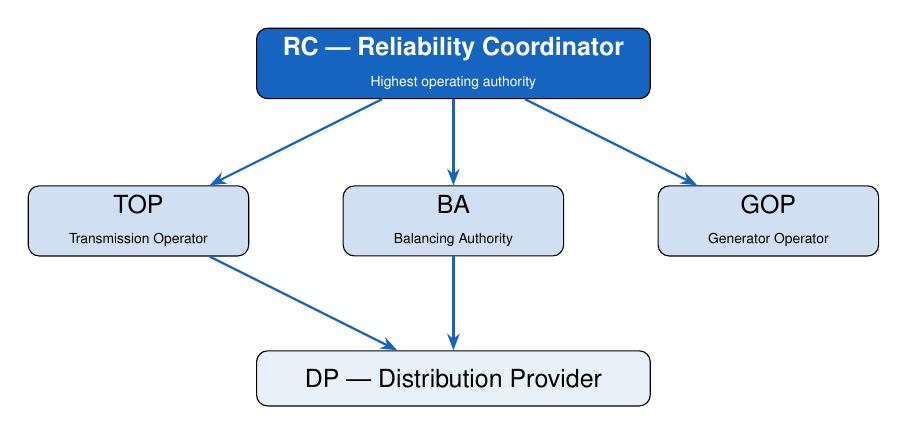
\begin{tikzpicture}[
  every node/.style={draw, rounded corners=4pt, align=center, font=\sffamily\small},
  arrow/.style={-{Stealth[length=6pt]}, thick, nercblue},
]
  \node[fill=nercblue, text=white, minimum width=5cm, minimum height=0.8cm]
    (rc) at (0,0) {\textbf{RC — Reliability Coordinator}\\{\tiny Highest operating authority}};

  \node[fill=nercblue!20, minimum width=2.8cm, minimum height=0.8cm]
    (top) at (-4,-2) {TOP\\{\tiny Transmission Operator}};
  \node[fill=nercblue!20, minimum width=2.8cm, minimum height=0.8cm]
    (ba) at (0,-2) {BA\\{\tiny Balancing Authority}};
  \node[fill=nercblue!20, minimum width=2.8cm, minimum height=0.8cm]
    (gop) at (4,-2) {GOP\\{\tiny Generator Operator}};

  \node[fill=nercblue!10, minimum width=5cm, minimum height=0.7cm]
    (dp) at (0,-4) {DP — Distribution Provider};

  \draw[arrow] (rc) -- (top);
  \draw[arrow] (rc) -- (ba);
  \draw[arrow] (rc) -- (gop);
  \draw[arrow] (top) -- (dp);
  \draw[arrow] (ba) -- (dp);
\end{tikzpicture}
\end{center}

\section{IRO-001-4: RC Authority}

Under IRO-001-4, the RC:
\begin{itemize}
  \item Shall take corrective actions to maintain the reliability of its RC Area
  \item Shall issue Operating Instructions to subordinate entities (TOPs, BAs, GOPs, DPs)
  \item Shall coordinate with adjacent RCs when wide-area conditions require it
\end{itemize}

Subordinate entities must:
\begin{itemize}
  \item Comply with RC Operating Instructions
  \item \textbf{Immediately inform the RC if they cannot comply}—silence is a violation
  \item Coordinate planned outages with the RC in advance
\end{itemize}

% ============================================================
\chapter{Interchange Scheduling}
\label{ch:interchange}
% ============================================================

\section{E-Tag Required Elements}

\begin{center}
\begin{tabular}{@{}lp{9cm}@{}}
\toprule
\rowcolor{nercblue!15}
\textbf{Element} & \textbf{Description} \\
\midrule
MW Amount & The amount of energy to be transferred \\
\rowcolor{rowlight}
Start/End Time & Operating period for the interchange \\
Ramp Time and Rate & Beginning/ending ramp times and MW/min rate \\
\rowcolor{rowlight}
Type of Service & Firm or Non-Firm for delivery and receipt \\
Source and Sink & Generating resource and receiving load area \\
\rowcolor{rowlight}
Transmission Path & The path over which the energy flows \\
\bottomrule
\end{tabular}
\end{center}

\section{INT-006-5: Reliability Adjustment}

\begin{examtip}
When the RC directs modification of Confirmed or Implemented Interchange for
reliability reasons, a Reliability Adjustment Arranged Interchange schedule must
be submitted within \textbf{60 minutes} of the start of the modification.
This is a frequently tested timing requirement.
\end{examtip}

% ============================================================
\chapter{Power Systems Fundamentals}
\label{ch:powersystems}
% ============================================================

\section{Governor Droop Response}

\begin{formulabox}{Governor Droop Calculation}
\[
\Delta\text{MW} = \frac{\text{Frequency Deviation (\%)}}{\text{Droop (\%)}} \times \text{Unit Rating (MW)}
\]

\textbf{Example:} 5\% droop, 100 MW unit, frequency drops from 60.00 to 59.70 Hz
\[
\text{Deviation} = \frac{0.30}{60} \times 100\% = 0.5\%
\quad\Rightarrow\quad
\Delta\text{MW} = \frac{0.5\%}{5\%} \times 100\,\text{MW} = 10\,\text{MW}
\]
\end{formulabox}

\section{Three Levels of Frequency Control}

\begin{description}
  \item[Primary (seconds):] Autonomous governor response, proportional to frequency
        deviation. Arrests frequency decline but does not restore 60 Hz.
  \item[Secondary (minutes):] AGC adjusts unit setpoints to eliminate ACE and restore
        frequency to scheduled value (60 Hz normally).
  \item[Tertiary (10--30 min):] Reserve restoration—start additional units, arrange
        emergency assistance, replenish contingency reserves.
\end{description}

% ============================================================
\chapter{Voltage \& Reactive Power}
\label{ch:var}
% ============================================================

\section{MVAR Sources and Sinks}

\begin{center}
\begin{tabular}{@{}ll@{}}
\toprule
\rowcolor{nercblue!15}
\textbf{Device/Condition} & \textbf{Effect on MVAR} \\
\midrule
Overexcited generator & Produces MVAR (raises voltage) \\
\rowcolor{rowlight}
Underexcited generator & Absorbs MVAR (lowers voltage) \\
Capacitor bank & Produces MVAR (raises voltage) \\
\rowcolor{rowlight}
Shunt reactor & Absorbs MVAR (lowers voltage) \\
Heavily loaded line & Consumes MVAR (drops receiving-end voltage) \\
\rowcolor{rowlight}
SVC / STATCOM & Adjustable MVAR injection or absorption \\
\bottomrule
\end{tabular}
\end{center}

\section{VAR Standards Summary}

\begin{description}
  \item[\std{VAR-001-6}:] Transmission Operator establishes voltage schedules or
        reactive power output schedules for generators at their interconnection points.
  \item[\std{VAR-002-4}:] Generator Operators must maintain terminal voltage or reactive
        output within schedules set by the TOP. If unable to comply, must immediately notify the TOP.
\end{description}

% ============================================================
\chapter{Practice \& Exam Strategy}
\label{ch:lab}
% ============================================================

\section{Critical Numbers Reference}

\begin{center}
\begin{tabular}{@{}lll@{}}
\toprule
\rowcolor{nercblue!15}
\textbf{Value} & \textbf{Meaning} & \textbf{Standard} \\
\midrule
15 minutes & DRL recovery after contingency & BAL-002-3 \\
\rowcolor{rowlight}
90 minutes & Reserve restoration after contingency & BAL-002-3 \\
10 minutes & Spinning/Non-Spinning Reserve deployment & BAL-002-3 \\
\rowcolor{rowlight}
$\leq$ 30 minutes & Maximum IROL violation time (Tv) & NERC Glossary \\
60 minutes & Reliability Adjustment e-tag submission & INT-006-5 \\
\rowcolor{rowlight}
2 years & Blackstart personnel training cycle & EOP-005-3 \\
3 years & RC certification renewal cycle & NERC Cert Program \\
\rowcolor{rowlight}
36 hours & CE hours required for 3-year renewal & NERC Cert Program \\
60.02 Hz & Scheduled frequency, slow time error correction & BAL-004 \\
\rowcolor{rowlight}
59.98 Hz & Scheduled frequency, fast time error correction & BAL-004 \\
$\geq$ 100\% & CPS1 minimum performance standard & BAL-001-2 \\
\rowcolor{rowlight}
$\sim$59.3 Hz & Typical UFLS first step threshold & PRC-006 \\
\bottomrule
\end{tabular}
\end{center}

\section{Scenario Question Framework}

For every scenario-based question, apply this four-step framework:
\begin{enumerate}
  \item \textbf{Who has authority?} Identify the responsible entity: RC, TOP, BA, GOP.
        The RC has widest authority but directs, not operates, equipment.
  \item \textbf{What standard applies?} Map the scenario: frequency $\to$ BAL; voltage
        $\to$ VAR/EOP; overload $\to$ TOP/IRO; blackstart $\to$ EOP-005.
  \item \textbf{What is the required timeline?} Reference the table above. Timelines are
        frequently tested and often distinguish correct from incorrect answers.
  \item \textbf{What is the correct sequence?} Assess $\to$ coordinate $\to$ direct action.
        The RC rarely acts unilaterally—it assesses, then directs the appropriate entity.
\end{enumerate}

\begin{warningbox}
\textbf{Common Mistakes on the RC Exam:}
\begin{itemize}
  \item Selecting "shed load immediately" before assessing — RC assesses first
  \item Confusing ISO (market entity) with a NERC certification
  \item Mixing up fast/slow time error scheduled frequency values
  \item Forgetting the 10$\times$ factor in the ACE bias term
  \item Applying TLR procedures to the Western Interconnection (TLR is Eastern only)
\end{itemize}
\end{warningbox}

% ============================================================
\backmatter
% ============================================================

\chapter*{Quick Reference: Key Standards}

\begin{center}
\begin{tabular}{@{}lp{10cm}@{}}
\toprule
\rowcolor{nercblue!15}
\textbf{Standard} & \textbf{Topic} \\
\midrule
BAL-001-2 & CPS1/CPS2 real power balancing performance \\
\rowcolor{rowlight}
BAL-002-3 & Disturbance Control Standard — MSSC reserves, DRL, 15-min recovery \\
BAL-003-2 & Frequency response and bias settings \\
\rowcolor{rowlight}
BAL-005 & Balancing Authority control — AGC requirements \\
BAL-006 & Inadvertent interchange accounting \\
\rowcolor{rowlight}
COM-001 & Communications — primary and alternate paths \\
EOP-005-3 & System restoration from blackstart — 2-year training \\
\rowcolor{rowlight}
EOP-006-2 & System restoration coordination — RC role \\
EOP-011-2 & Emergency operations preparedness — TOPs maintain plans \\
\rowcolor{rowlight}
FAC-001 & Facility connection requirements \\
FAC-002 & Facility connections and planning analysis \\
\rowcolor{rowlight}
INT-006-5 & Interchange evaluation and reliability adjustment \\
INT-009-3 & RC interchange evaluation \\
\rowcolor{rowlight}
IRO-001-4 & RC authority — highest operating authority \\
IRO-006-EAST-2 & TLR procedures — Eastern Interconnection \\
\rowcolor{rowlight}
IRO-008-2 & Operational Planning Analysis (OPA) — next-day \\
IRO-017-1 & Wide-area situational awareness tools \\
\rowcolor{rowlight}
MOD-001 & Generator real and reactive capability data \\
PRC-006 & Under-Frequency Load Shedding (UFLS) \\
\rowcolor{rowlight}
TOP-001-5 & Transmission operations — SOL/IROL compliance \\
VAR-001-6 & Voltage and reactive control — TOP sets schedules \\
\rowcolor{rowlight}
VAR-002-4 & Generator reactive capability — GOPs follow TOP schedules \\
\bottomrule
\end{tabular}
\end{center}

\end{document}
